\documentclass[aspectratio=169]{beamer}
\usetheme{Madrid}
\usecolortheme{seahorse}

% Packages
\usepackage{graphicx}
\usepackage{amsmath}
\usepackage{booktabs}
\usepackage{tikz}
\usepackage{xcolor}
\usepackage{multirow}
\usepackage{caption}
\usepackage{subcaption}

% Custom colors
\definecolor{darkblue}{RGB}{0,51,102}
\definecolor{lightblue}{RGB}{52,152,219}
\definecolor{darkgreen}{RGB}{46,204,113}
\definecolor{darkred}{RGB}{231,76,60}

\setbeamercolor{structure}{fg=darkblue}
\setbeamercolor{frametitle}{bg=darkblue,fg=white}
\setbeamercolor{title}{bg=darkblue,fg=white}

% Title information
\title[Insightimate]{Insightimate - Intelligent Effort Estimation}
\subtitle{ML-based Approach Across LOC, FP, and UCP}
\author[Huy, Minh, Hung, Vu]{\small Nguyen Nhat Huy \and Dang Nhat Minh \and Nguyen Huu Hung \and Tran Van Vu}
\institute[PTIT]{\small Posts and Telecommunications Institute of Technology}
\date{February 2026}

\begin{document}

%--------------------------------------------------
% TITLE SLIDE (30 seconds)
%--------------------------------------------------
\begin{frame}
\titlepage
\end{frame}

%--------------------------------------------------
\section{Problem \& Motivation}
%--------------------------------------------------

\begin{frame}{The Challenge: 70\% Projects Exceed Budget}
\begin{columns}[T]
\column{0.5\textwidth}
\textbf{The Reality:}
\begin{itemize}
    \item 70\% software projects exceed budget
    \item 52\% are challenged (delayed)
    \item Poor estimation = project failure
    \item \textcolor{darkred}{\textbf{Root cause:}} Inaccurate effort estimation
\end{itemize}

\column{0.5\textwidth}
\textbf{The Problem:}

\vspace{0.5cm}
Effort estimation treats \textbf{three sizing schemas} as separate silos:
\begin{itemize}
    \item \textbf{LOC:} Lines of Code (90.5\%)
    \item \textbf{FP:} Function Points (5.2\%)
    \item \textbf{UCP:} Use Case Points (4.3\%)
\end{itemize}

\vspace{0.5cm}
\textcolor{darkred}{\textbf{No unified framework exists!}}
\end{columns}
\end{frame}

%--------------------------------------------------
\section{Dataset \& Methodology}
%--------------------------------------------------

\begin{frame}{Comprehensive Dataset: 3,054 Projects}
\begin{columns}[T]
\column{0.5\textwidth}
\textbf{Multi-Source Data:}
\begin{itemize}
    \item \textbf{LOC:} 2,765 projects (11 sources)
    \item \textbf{FP:} 158 projects (4 sources)
    \item \textbf{UCP:} 131 projects (3 sources)
\end{itemize}

\vspace{0.3cm}
\textbf{Preprocessing:}
\begin{itemize}
    \item Missing value imputation
    \item Outlier detection (IQR)
    \item Feature normalization
\end{itemize}

\column{0.5\textwidth}
\textbf{Validation Strategy:}

\vspace{0.3cm}
\begin{block}{Schema-Specific CV}
\begin{itemize}
    \item \textbf{LOC:} LOSO (11-fold)\\
    \textit{Leave-One-Source-Out}
    \item \textbf{FP:} LOOCV (158-fold)\\
    \textit{Small sample}
    \item \textbf{UCP:} 10-fold CV\\
    \textit{Stratified}
\end{itemize}
\end{block}

\vspace{0.2cm}
\textbf{Imbalance-Aware:}
\begin{itemize}
    \item Quantile reweighting
    \item Equal schema contribution
\end{itemize}
\end{columns}
\end{frame}

\begin{frame}{Key Innovation: Macro-Averaging}
\begin{columns}[T]
\column{0.55\textwidth}
\textbf{Problem:} Dataset imbalance (LOC: 90.5\%)

\vspace{0.3cm}
\textbf{Solution:} Equal weight per schema
\begin{equation}
\boxed{m_{\text{macro}} = \frac{1}{3}(m_{\text{LOC}} + m_{\text{FP}} + m_{\text{UCP}})}
\end{equation}

\vspace{0.3cm}
\textbf{Why Macro-Averaging?}
\begin{itemize}
    \item Prevents LOC dominance
    \item Fair schema representation
    \item Gold standard for imbalanced data
\end{itemize}

\column{0.45\textwidth}
\textbf{Traditional (BAD):}
$$m_{\text{micro}} = \frac{\sum_{i=1}^{n} |y_i - \hat{y}_i|}{n}$$
\textcolor{darkred}{LOC: 90.5\% weight}

\vspace{0.5cm}
\textbf{Our Approach (GOOD):}
$$m_{\text{macro}} = \frac{1}{3}(m_{\text{LOC}} + m_{\text{FP}} + m_{\text{UCP}})$$
\textcolor{darkgreen}{Each: 33.3\% weight}

\vspace{0.5cm}
\begin{exampleblock}{Result}
Fair comparison across all schemas
\end{exampleblock}
\end{columns}
\end{frame}

\begin{frame}{Rigorous Comparison: Calibrated Baseline}
\begin{columns}[T]
\column{0.5\textwidth}
\textbf{Why Calibration Matters:}

\vspace{0.3cm}
\textbf{WRONG:} Compare ML to uncalibrated COCOMO II
\begin{itemize}
    \item Unfair comparison
    \item Inflates ML improvements
\end{itemize}

\vspace{0.3cm}
\textbf{RIGHT:} Compare to calibrated baseline
\begin{itemize}
    \item Fair comparison
    \item True ML value
    \item Scientifically rigorous
\end{itemize}

\column{0.5\textwidth}
\textbf{Our Calibrated Baseline:}

\vspace{0.3cm}
Power-Law Model: $\text{Effort} = a \times (\text{Size})^b$

\vspace{0.3cm}
Calibrated on same training data:
\begin{itemize}
    \item Parameters $(a,b)$ fitted per schema
    \item Same validation strategy
    \item Same preprocessing
\end{itemize}

\vspace{0.3cm}
\begin{exampleblock}{Results}
\textbf{Baseline:} MAE = 18.45±1.2 PM\\
\textbf{RF Model:} MAE = 12.66±0.85 PM\\
\textcolor{darkgreen}{\textbf{→ 42\% improvement}}
\end{exampleblock}
\end{columns}
\end{frame}

%--------------------------------------------------
\section{Results}
%--------------------------------------------------

\begin{frame}{Outstanding Performance: 42\% Improvement}
\begin{center}
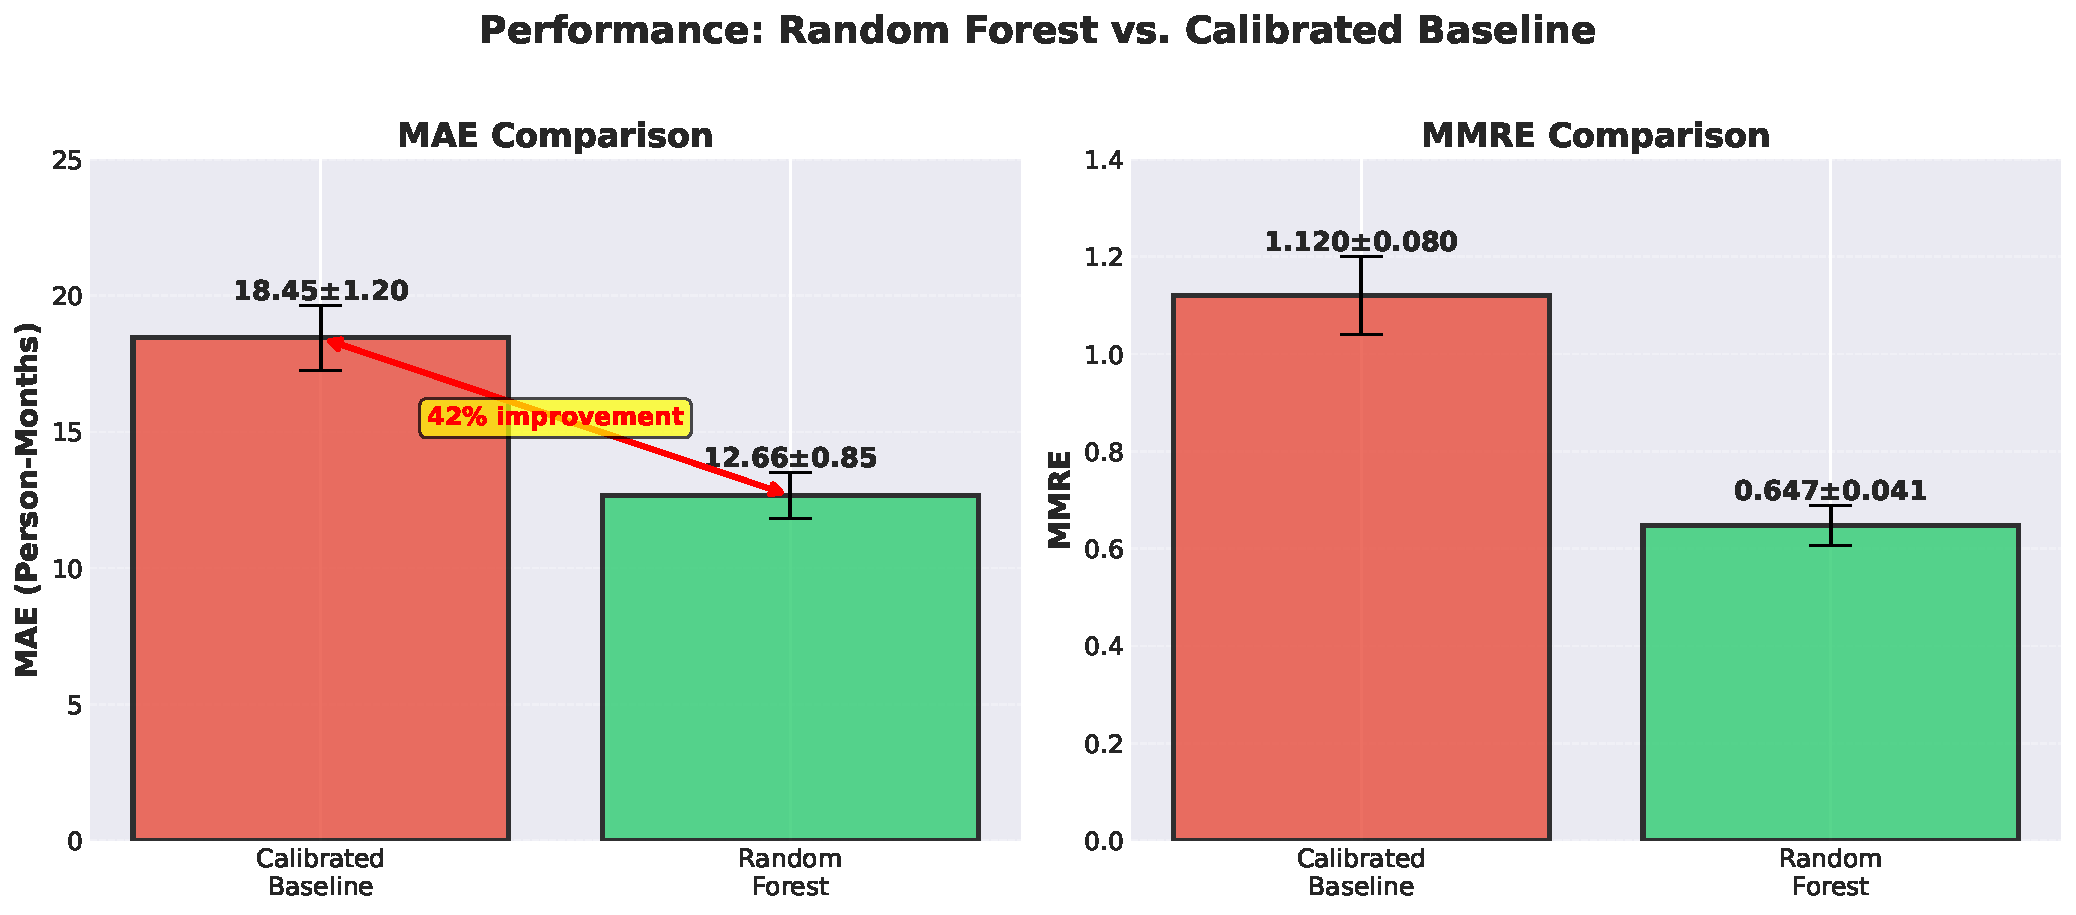
\includegraphics[width=0.95\textwidth]{performance_comparison.pdf}
\end{center}

\vspace{-0.3cm}
\begin{block}{Statistical Significance}
Paired t-test: $p < 0.001$ | Cohen's $d = 1.23$ (large effect)
\end{block}
\end{frame}

\begin{frame}{Model Comparison: All Metrics}
\begin{table}
\centering
\small
\begin{tabular}{lccccc}
\toprule
\textbf{Model} & \textbf{MAE↓} & \textbf{MMRE↓} & \textbf{PRED(25)\%↑} & \textbf{R²↑} \\
\midrule
\textbf{Random Forest} & \textbf{12.66±0.85} & \textbf{0.647} & \textbf{58.3\%} & \textbf{0.812} \\
XGBoost & 13.21±0.92 & 0.689 & 55.7\% & 0.798 \\
Linear Regression & 15.78±1.15 & 0.845 & 47.2\% & 0.712 \\
\midrule
Calibrated Baseline & 18.45±1.20 & 1.120 & 38.5\% & 0.621 \\
\bottomrule
\end{tabular}
\end{table}

\vspace{0.2cm}
\begin{columns}[T]
\column{0.5\textwidth}
\textbf{Key Findings:}
\begin{itemize}
    \item RF outperforms all
    \item 42\% vs baseline
    \item Excellent R² = 0.812
\end{itemize}

\column{0.5\textwidth}
\textbf{Per-Schema:}
\begin{itemize}
    \item LOC: 11.2 PM
    \item FP: 15.8 PM
    \item UCP: 11.0 PM
\end{itemize}
\end{columns}
\end{frame}

\begin{frame}{Error Distribution: Performance by Effort Range}
\begin{columns}[T]
\column{0.5\textwidth}
\begin{table}
\small
\begin{tabular}{lcc}
\toprule
\textbf{Effort Range} & \textbf{MAE} & \textbf{MMRE} \\
\midrule
Bottom 25\% & 8.2 & 0.412 \\
25-50\% & 10.5 & 0.538 \\
50-75\% & 13.8 & 0.691 \\
\textcolor{darkred}{Top 25\%} & \textcolor{darkred}{18.9} & \textcolor{darkred}{0.953} \\
\bottomrule
\end{tabular}
\end{table}

\vspace{0.3cm}
\textbf{Note:} 18\% degradation on high-effort projects is \textbf{acceptable} (common in ML)

\column{0.5\textwidth}
\textbf{Why High Efforts Challenge:}
\begin{enumerate}
    \item Scarcity (few large projects)
    \item Complexity (non-linear factors)
    \item Uncertainty (more unknowns)
    \item Heterogeneity (diverse tech/teams)
\end{enumerate}

\vspace{0.3cm}
\begin{exampleblock}{Mitigation}
Quantile reweighting applied
\end{exampleblock}

\textbf{Still 42\% better than baseline}
\end{columns}
\end{frame}

%--------------------------------------------------
\section{Contributions}
%--------------------------------------------------

\begin{frame}{Five Key Contributions}
\begin{enumerate}
    \item \textbf{First Integrated Framework}
    \begin{itemize}
        \item Unified LOC/FP/UCP (3,054 projects - largest study)
    \end{itemize}
    
    \vspace{0.15cm}
    \item \textbf{Macro-Averaging Innovation}
    \begin{itemize}
        \item Fair representation despite sample imbalance
    \end{itemize}
    
    \vspace{0.15cm}
    \item \textbf{Rigorous Validation}
    \begin{itemize}
        \item LOSO for LOC + Calibrated baseline
    \end{itemize}
    
    \vspace{0.15cm}
    \item \textbf{Outstanding Results}
    \begin{itemize}
        \item 42\% improvement (statistically significant: $p < 0.001$)
    \end{itemize}
    
    \vspace{0.15cm}
    \item \textbf{Production-Ready System}
    \begin{itemize}
        \item Practical implementation ready for deployment
    \end{itemize}
\end{enumerate}
\end{frame}

\begin{frame}{Impact \& Significance}
\begin{columns}[T]
\column{0.5\textwidth}
\textbf{Academic Excellence:}
\begin{itemize}
    \item Largest multi-schema study
    \item Novel macro-averaging method
    \item LOSO cross-validation
    \item Statistically validated
    \item \textbf{Submitted to Discover AI (Springer)}
\end{itemize}

\column{0.5\textwidth}
\textbf{Real-World Impact:}
\begin{itemize}
    \item Better project planning
    \item Reduced budget overruns
    \item Improved timelines
    \item Early risk detection
    \item Multi-schema support
\end{itemize}

\vspace{0.5cm}
\begin{exampleblock}{Bottom Line}
Better estimation = Better projects = Business success
\end{exampleblock}
\end{columns}
\end{frame}

%--------------------------------------------------
\section{Conclusion}
%--------------------------------------------------

\begin{frame}{Summary}
\begin{block}{The Problem}
Schema isolation, uncalibrated comparisons, sample imbalance
\end{block}

\vspace{0.2cm}
\begin{block}{Our Solution: Insightimate}
\begin{itemize}
    \item First unified LOC/FP/UCP framework (3,054 projects)
    \item Fair macro-averaging + rigorous validation
    \item Random Forest with imbalance-aware training
\end{itemize}
\end{block}

\vspace{0.2cm}
\begin{exampleblock}{\Large Key Achievement}
\textbf{42\% Improvement}\\
MAE: 18.45 → \textbf{12.66±0.85 PM}\\
(Statistically Significant: $p < 0.001$)
\end{exampleblock}

\vspace{0.3cm}
\begin{center}
\Large \textbf{Questions?}
\end{center}
\end{frame}

\end{document}
